% =============================================================================
% Paper 05: audit and correction record of the TinkerRL run corpus
% Root: platform_hybrid/paper/paper.tex (descendant of NeurIPS submission #36320)
% =============================================================================
% Template: NeurIPS 2026 style file (neurips_2026.sty), used for layout only.
% Retarget (2026-10-19 ARS revision): short audit / correction note for a
% reproducibility, audit, or workshop venue. The target venue, its page budget,
% and its anonymity rules are author decisions and are not fixed here.
% Build: tectonic -X compile paper.tex (status and build record:
% reports/ars_review_2026-10-19/corrections/05_status.md).
% Gates: python3 platform_hybrid/paper/scripts/p05_ledger_window_gate.py
%        python3 platform_hybrid/paper/scripts/p05_build_reviewed_cells_manifest.py
% =============================================================================
% SUBMISSION NOTE: for an anonymous build, compile a scratch wrapper that
% defines \paperauditsubmission before inputting this file, and replace
% repository/Hub URLs with an anonymized mirror. Inspect the rendered PDF;
% the switch does not certify anonymity.

\documentclass{article}

\ifdefined\paperauditsubmission
  \usepackage[nonatbib]{neurips_2026}
\else
  \usepackage[preprint,nonatbib]{neurips_2026}
\fi
\usepackage[numbers]{natbib}

\usepackage[utf8]{inputenc}
\usepackage[T1]{fontenc}
\usepackage{hyperref}
\hypersetup{hidelinks}
\usepackage{xurl}
\usepackage{booktabs}
\usepackage{amsfonts}
\usepackage{amsmath}
\usepackage{amssymb}
\usepackage{nicefrac}
\usepackage{microtype}
\usepackage{xcolor}
\usepackage{graphicx}
\usepackage{enumitem}

% Custom commands
\newcommand{\tinker}{\textsc{Tinker}}
\newcommand{\atropos}{\textsc{Atropos}}
\newcommand{\grpo}{\textsc{Grpo}}
\newcommand{\ours}{\textsc{TinkerRL Audit}}

\title{An Evidence Audit and Correction Record for Critic-Free Group-Relative
RL Runs: Homogeneous-Reward Groups, Window Labels, and Artifact Identity}

\author{
  Arvind C R\thanks{Equal contribution.} \\
  PES University\\
  \texttt{arvindcr4@gmail.com} \\
  \And
  Sandhya Jeyaraj\footnotemark[1] \\
  PES University\\
  \texttt{sandhya.jeyaraj2014@gmail.com} \\
  \And
  Madhu Kumara L \\
  PES University\\
  \texttt{madhukumara1993@gmail.com} \\
  \And
  Mohammad Rafi \\
  PES University\\
  \texttt{gmd.rafi.2024@gmail.com} \\
  \And
  Dhruva N Murthy \\
  PES University\\
  \texttt{dhruva.n.murthy@gmail.com} \\
  \And
  Arumugam K \\
  PES University\\
  \texttt{chettyarumugam@mail.com} \\
  \And
  Anwesh Reddy Paduri \\
  Great Learning / PES University\\
  \texttt{anwesh@greatlearning.in} \\
  \And
  Narayana Darapaneni \\
  Northwestern University / Great Learning\\
  \texttt{narayana.darapaneni@northwestern.edu} \\
}

% Custom command for partial answers in NeurIPS checklist
\newcommand{\answerPartial}[1][]{\textcolor{purple}{[Partial] #1}}

\begin{document}

\maketitle

% Paper-05-only abstract and introduction (forked from the shared
% sections/abstract.tex and sections/intro.tex, which the archived U01 roots use).
% =============================================================================
% Abstract for paper 05 only (platform_hybrid/paper/paper.tex).
% Forked 2026-10-19 from sections/abstract.tex, which is also consumed by the
% archived U01 compendium root; edit this file, not the shared one.
% =============================================================================
\begin{abstract}
Critic-free group-relative RL centres each completion's reward on its group
mean, so a prompt whose completions all receive the same reward contributes no
centred reward contrast. This is an audit and correction record of one
heterogeneous run corpus, not a new algorithm, benchmark, diagnostic, or
algorithm ranking. We report three things. First, for the specified
noncanonical runner (no ratio/clipping, reference-KL, or completion-only mask)
homogeneous rewards make the centred reward-contrast term exactly zero; this
does not imply a zero total gradient and does not transfer to canonical GRPO.
Second, the two reviewed synthetic tool-use cells have reward 0 and
zero-variance fraction (ZVF) 1 at every logged step, with no held-out
evaluation; they are descriptive all-wrong cases whose cause (policy, parser,
or prompt template) is not identified, and they validate no predictor,
triage rule, or stopping policy. Third, an artifact-bound re-audit of the
training-reward ledger corrects window labels, quarantines rows whose
artifacts conflict, and withdraws untraced summaries. We do not test whether
reward contrast rather than algorithm labels explains cross-stack gaps.
\end{abstract}

% Introduction for paper 05 only (platform_hybrid/paper/paper.tex).
% Forked 2026-10-19 from sections/intro.tex, which is also consumed by the
% archived U01 compendium roots; edit this file, not the shared one.
\section{Introduction}
\label{sec:intro}
Comparing RL post-training systems requires separating the algorithm name from
the implemented objective, sampling protocol, checkpoint, and evaluator.
Implementation sensitivity is already established in policy-gradient
research~\citep{engstrom2020implementation,henderson2018deep}; heterogeneous
observations alone do not identify which implementation choice caused a gap.

This manuscript is a bounded audit of one run corpus. Its contributions are:
\begin{enumerate}
\item An objective-scoped account of why homogeneous rewards eliminate the
centred reward-contrast term in the specified noncanonical runner
(Section~\ref{sec:diagnostic-method}).
\item An artifact-bound inventory of the two reviewed synthetic tool-use cells,
with an immutable manifest and the alternative explanations it cannot exclude
(Section~\ref{sec:evidence-identity}).
\item A re-audit of the training-reward ledger under one standard: every
retained number is bound to a named artifact and a correctly labelled window,
or it is quarantined or withdrawn (Section~\ref{sec:main_results}).
\end{enumerate}
These contributions do not include a new diagnostic definition, a controlled
cross-library benchmark, a validated predictor, triage rule, or stopping rule,
or an algorithm ranking.

\paragraph{Relation to existing zero-advantage diagnostics.}
The fraction of groups with zero reward variance is already an operational
quantity in group-relative RL: AVSPO's Advantage Collapse Rate measures the
same object up to a tolerance~\citep{he2026advantage}, and dynamic sampling in
DAPO~\citep{yu2025dapo} and variance- or pass-rate-based prompt selection
(e.g., VCRL~\citep{jiang2025vcrl}) act on it. We therefore use the name
Zero-Variance Fraction (ZVF) only as a reporting field and claim no new
measurable, estimator, or intervention. Its complement is called the
\emph{mixed-group fraction} here (historical alias: Gradient Utilization, GU);
it measures only the fraction of groups with nonconstant rewards, not gradient
magnitude or usefulness. For binary rewards it should be reported signed
(all-wrong, all-correct, mixed) rather than as one number.

\paragraph{Why an audit.}
The corpus was assembled for an earlier, broader manuscript. Re-checking its
displays against the stored artifacts showed mislabelled windows, rows whose
two artifact versions disagree, and summaries with no released source
(Section~\ref{sec:main_results}). Readers of any text that reuses this corpus
need those dispositions; the relationship to those texts is mapped in
Section~\ref{sec:overlap}.

% Paper 05 only: overlap and disclosure map (ARS 2026-10-19 EIC-W3 / DA-MAJOR-3).
\section{Relationship to Other Texts From the Same Corpus}
\label{sec:overlap}

This manuscript descends from NeurIPS submission \#36320 but is
not its authenticated or byte-identical reviewed PDF; we audit that submitted record
rather than claiming that local edits change it. The same run corpus is also
used by an associated thesis and by sibling manuscripts. Table~\ref{tab:overlap}
lists, for each display of this audit, the other texts in the repository whose
source contains the same values. The scan is a string-level search of each
root's \LaTeX{} inclusion closure (and of the thesis chapter sources) for
display-specific values; it detects reuse of these numbers, not paraphrase or
reuse of other material, and it does not establish submission status.

\begin{table}[htbp]
\centering\scriptsize
\caption{Overlap map for the displays of this audit (2026-10-19 scan). P1--P12
are the live sibling roots listed in
\texttt{platform\_hybrid/paper/scripts/publication\_worthiness\_check.py}; the
thesis is \texttt{reports/public\_revision\_2026-10-11/thesis/}. ``None found''
means the probe values were absent, not that the texts are unrelated.}
\label{tab:overlap}
\begin{tabular}{@{}p{.30\linewidth}p{.33\linewidth}p{.27\linewidth}@{}}
\toprule
Display in this audit & Same values also in & Unique here \\
\midrule
Two reviewed tool-use cells (Table~\ref{tab:audited-tool-cells}) & P2, P6, P9; thesis ch.~7, 10 & Manifest and alternative-explanation audit \\
Held-out GSM8K five-adapter check (Section~\ref{sec:heldout}) & P8, P9; thesis ch.~1, 6, 7, 10 & Prompt-paired discordance counts \\
Wave~6 sensitivity sweep & P5, P8, P9 & None \\
Task~4 stack-sensitivity rows & P5, P6, P7, P9 & None \\
Nemotron-120B trace (87.5\% peak, 16.2\% last-10) & P8 & None \\
Training-reward ledger re-audit (Table~\ref{tab:main_results}) & Individual rows in several siblings & Window corrections and conflict quarantines \\
Withdrawn summaries (SI/PTD, lagged ZVF, team percentages) & --- & Withdrawal record \\
\bottomrule
\end{tabular}
\end{table}

\paragraph{Disclosure.}
No display here should be counted as evidence independent of the same rows in a
sibling text. The thesis Table~6.2 remains provisional; this audit does not
change its numbers or upgrade its status. The portfolio companions on
terminal-signal decision analysis (\path{zvf-program/flagship/paper/main.tex}),
receipt-bound evaluation governance (\path{papers/icicc2027/paper_camera.tex}),
stack-conditioned measurement
(\path{papers/pes_ieee_attribution/ArvindCR_GRPO_Attribution_IEEE.tex}), and
zero-advantage spectral analysis
(\path{papers/spectral_entropy_grpo/spectral_entropy_paper_kdense_revision.tex})
share the zero-advantage background but none of the probe values above. Which of these texts is, or will be, under review at
any venue must be declared by the authors at submission; it is not asserted here.

% Paper 05 only: related work cut to the load-bearing lineage (ARS 2026-10-19,
% R2-W1 / R2-W3). Sentences are condensed from sections/related_work_v2.tex
% (shared with archived roots, left unchanged); quoted external effect sizes
% are dropped rather than repeated unverified.
\section{Related Work}
\label{sec:related}

\paragraph{Zero-advantage diagnostics and interventions.}
Recent work pre-empts the diagnostic used here. The Advantage Collapse Rate
(ACR) of AVSPO~\cite{he2026advantage} measures the same homogeneous-group
advantage collapse that we call ZVF (ACR thresholds reward SD while ZVF uses
exact equality; matching thresholds and prompt weights makes the measured
object coincide) and reports that it predicts stagnation and final performance;
Gradient Starvation~\cite{nie2026gradstarvation} shows that the true degeneracy
rate exceeds the i.i.d.\ Bernoulli prediction by Jensen's inequality.
DAPO~\cite{yu2025dapo} discards homogeneous groups through dynamic sampling;
VCRL~\cite{jiang2025vcrl} and online difficulty filtering~\cite{bae2025online}
select prompts by group reward variance or intermediate pass rate;
GRESO~\cite{zhang2026greso} pre-screens prompts before sampling;
CPPO~\cite{lin2025cppo} prunes completions after rollout;
NGRPO~\cite{nan2025ngrpo} calibrates advantages so that all-incorrect groups
still carry gradient; query recycling treats zero-variance queries as
candidates for later resampling~\cite{coelho2026recycling}; and
AERO~\cite{zhang2026aero} pre-screens prompts with a posterior over difficulty.
These are prior or concurrent diagnostics and interventions, not evidence for
the audited runner. Relative to them this audit adds no measurable, estimator,
or intervention; it contributes a correction record and the requirement that
the fraction be reported signed and bound to a cohort.

\paragraph{Objective variants.}
GRPO was introduced with DeepSeekMath~\cite{shao2024deepseekmath}.
Dr.~GRPO~\cite{tong2025drgrpo} removes a response-length bias and a
question-difficulty bias by using a constant loss normaliser and dropping the
standard-deviation denominator; GSPO~\cite{qwen2025gspo} defines the importance
ratio at the sequence level; Wu et al.~\cite{wu2025grpodpo} relate GRPO and DPO
through contrastive-gradient representations; and TPO~\cite{kaddour2026tpo}
targets a tilted distribution whose homogeneous-group first-epoch
reward-directed gradient is zero at the rollout snapshot. The audited runner is
none of these (Section~\ref{sec:diagnostic-method}).

\paragraph{Implementation sensitivity and reporting.}
Implementation Matters~\cite{engstrom2020implementation} and Henderson et
al.~\cite{henderson2018deep} document how implementation choices and seeds move
apparent policy-gradient gains; \texttt{rliable}~\cite{agarwal2021deep}
introduced interval estimates and performance profiles for few-run reporting;
and controlled multi-algorithm studies on shared infrastructure find
scale-dependent ranking inversions~\cite{li2026oxrl}. Verifier errors and
evaluation artefacts can inflate apparent reasoning gains~\cite{zhang2025verifybench,
hochlehnert2025sober}. Framework defaults (TRL~\cite{vonwerra2022trl},
OpenRLHF~\cite{hu2024openrlhf}, veRL~\cite{sheng2024verl},
\tinker{}~\cite{thinkingmachines2024tinker}) differ in advantage
normalisation, KL estimators, loss masking, rollout batching, and
importance-sampling granularity; these are possible confounders of any
cross-stack row here, not identified causes. Pineau et
al.~\cite{pineau2020improving} and ACM Artifact Review and
Badging~\cite{acm2020badges} supply the reproducibility vocabulary used in
Section~\ref{sec:reproducibility}.


% =============================================================================
% Reviewed-record descendant: method and scope before corpus results.
\section{Diagnostic Method and Objective Scope}
\label{sec:diagnostic-method}

For a prompt with a sampled group of rewards, the submitted runner centers each
reward by the group mean. If all rewards are homogeneous, every centered
reward-contrast coefficient is zero; hence the submitted reward-contrast term
is zero. We call the fraction of such groups ZVF and write its submitted
complement as Gradient Utilization, $\mathrm{GU}=1-\mathrm{ZVF}$. GU measures the fraction of groups with nonconstant rewards. Mixed rewards
guarantee nonzero centered coefficients, not a nonzero aggregate gradient,
correct reward information, or learning progress: contributions can cancel, masks
can suppress them, and an erroneous verifier can supply contrast. This is an
accounting identity for this runner, not a measurement of a total optimizer gradient.

The diagnostic runner is \emph{not canonical GRPO}. It was deliberately minimal
for a narrow audit of centered rewards: it omits a PPO probability ratio and
clipping, frozen-reference KL, and completion-only token masking. Those omissions
do not make the omitted terms irrelevant. Clipping and completion-only masking can
change which token contributions survive, while reference KL or auxiliary losses
can make the total gradient nonzero even when the centered reward-contrast term is
zero. The results therefore neither establish canonical-GRPO equivalence nor
transfer to a different objective.

We organize observations by evidence tier and estimand rather than pooling
heterogeneous models, tasks, runners, checkpoints, and evaluators as replications.
In the reviewed record, the two synthetic tool-use cells have reward 0, ZVF 1,
GU 0, and held-out outcome \emph{not evaluated}; GSM8K ZVF is only a heterogeneous
descriptive aggregate unless a named per-run source is given. Later files such as
\texttt{zvf\_iter70\_per\_run\_zvf\_acc.tsv} are future-paper evidence and do not
repair the reviewed record. Under binary rewards, high-reward/high-ZVF is a
theoretical solved-task regime, not an observed claim here: it yields zero centered
contrast, may waste rollout budget, and cannot by unsigned ZVF alone choose
retire/distill over retry/resample/warm-start.

\paragraph{Local objective specification and provenance.}
The legacy local implementation at repository commit \texttt{ddcbb868}, in
\path{platform_hybrid/experiments/tinker-runs/scripts/grpo_exp_a_baseline.py}
(function \texttt{grpo\_loss\_fn} and its group loop), computes
\begin{align}
\bar r_q&=G^{-1}\sum_i r_{qi},\qquad
s_q=\sqrt{G^{-1}\sum_i(r_{qi}-\bar r_q)^2},\\
a_{qi}&=\operatorname{stopgrad}\left[(r_{qi}-\bar r_q)/(s_q+10^{-8})\right],\\
L_{\mathrm{local}}&=-\frac{1}{M}\sum_{q,i}a_{qi}
 \sum_{j=1}^{T_{qi}}\ell_{qij}(\theta).
\end{align}
Here $M$ counts collected completions; grouping is per sampled prompt, the SD
uses divisor $G$, and scalar rewards/advantages are computed outside autograd.
The callback sums all returned token log-probabilities before averaging over
completions; it does not length-normalize or apply completion-only token masking.
The legacy target construction shifts the concatenated prompt/response token
sequence and appends a dummy zero target. Thus $\ell$ denotes the callback's
returned log-probabilities, not a claimed correctly masked conditional-completion
likelihood. There is no ratio, clipping, or local reference-KL term in this loss.
Backend optimizer state and any unobserved terms are outside the identity.

This source snapshot is evidence of local implementation semantics, not proof
that a particular reviewed execution used that exact commit. Later corrected
alignment/masking code must not be projected onto historical runs. The two
reviewed cell-to-execution mappings remain incomplete.
For binary rewards, report all-wrong, all-correct, and mixed group fractions
separately. For graded schema rewards, also identify homogeneous intermediate
scores; binary Bernoulli formulas do not apply to that entire reward scale.
Exact equality defines ZVF here; any tolerance-based variant must declare its
threshold, grouping weights, and treatment of missing/nonfinite rewards.


% =============================================================================
\section{Audit Corpus and Evidence Design}
\label{sec:benchmark}
% =============================================================================

The corpus contains three task families with reported observations
(Table~\ref{tab:tasks}). Rewards are computed by deterministic parsers rather
than learned reward models: binary final-answer matching for GSM8K and the
arithmetic task, and a graded schema score for tool use (Section~\ref{sec:evidence-identity})
that does not execute tools. Verifiable rewards reduce reliance on reward models
but can still be gamed through parser artifacts, format shortcuts, and length
effects. Library mappings and configuration-only inventories from the earlier
manuscript are listed in Appendix~\ref{app:archive}.

\begin{table}[htbp]
\centering
\caption{Task families with reported observations in this audit. ``Audited
runner'' is the noncanonical group-relative runner of
Section~\ref{sec:diagnostic-method}.}
\label{tab:tasks}
\small
\begin{tabular}{@{}p{.27\linewidth}p{.25\linewidth}p{.22\linewidth}p{.16\linewidth}@{}}
\toprule
\textbf{Task} & \textbf{Treatment} & \textbf{Reward} & \textbf{Prompts} \\
\midrule
Synthetic tool use (reviewed cells) & Audited runner & Graded JSON-schema score & 10 in-source prompts \\
Math RL (GSM8K) & Audited runner; TRL-GRPO; PPO & Binary final answer & GSM8K train/test \\
Math RL (arithmetic) & Classic-RL PPO; TRL-GRPO & Binary correctness & Generated \\
\bottomrule
\end{tabular}
\end{table}

\begin{table}[htbp]
\centering
\caption{Evidence types and permitted interpretations in this audit.}
\label{tab:evidence_types_detail}
\scriptsize
\begin{tabular}{p{3.2cm}p{3.0cm}p{2.5cm}p{2.5cm}}
\toprule
\textbf{Evidence type} & \textbf{Runs} & \textbf{Independent unit} & \textbf{Can support} \\
\midrule
Audited-runner traces (Tinker) & Single runs, 3--30 logged steps & run & descriptive dynamics only \\
GSM8K held-out base vs.\ adapters & 5 adapters, 200 prompts & one-sample seed-level vs.\ fixed baseline & narrow capability check; inconclusive \\
Reviewed tool-use cells & 2 runs, 30 steps & run & descriptive all-wrong cases \\
Team proxy experiments & untraced & none bound & nothing (withdrawn) \\
\midrule
\multicolumn{4}{p{11.2cm}}{\small \textit{Note:} step-level rewards inside one training trace are autocorrelated telemetry, not independent observations. Any inferential test must name an independent seed, prompt, or replicated-run unit and its dependence assumptions.} \\
\bottomrule
\end{tabular}
\end{table}

% =============================================================================
\section{Experimental Setup}
\label{sec:setup}
% =============================================================================

\paragraph{Models and platforms.}
Models are listed per row in Table~\ref{tab:main_results}; the corpus spans
Qwen3, Qwen3.5, Llama-3.x, DeepSeek-V3.1, Nemotron-3-Super-120B-A12B (a sparse
model with about 12B active parameters), GPT-OSS, and Kimi checkpoints, run
either through the managed Tinker API (LoRA training with a local custom loss)
or on Modal H100s (TRL-GRPO and PPO). No single reconciled run total is
claimed.

\paragraph{Training protocol.}
LoRA~\cite{hu2022lora} settings vary by cohort: the scale, MoE, and tool-use
rows use rank 32, learning rate $3\times10^{-5}$, and $G=8$; the frontier and
``Kimi-K2'' rows use rank 16, $10^{-5}$, and $G=4$; the campaign~v2 rows use
$10^{-5}$ and $G=8$ unless the row states $G$; Wave~6 uses rank 32 by default,
$10^{-5}$, and $G=8$. Per-run values are in the cited artifacts.
Only the GSM8K held-out evaluation has five adapters; every Tinker training row
in the ledger is a single run with seed 42.

\subsection{Statistical Methodology}
\label{sec:statistical-policy}
Training steps within a run are autocorrelated and may be nonstationary. We
retain fixed-window summaries and descriptive coefficients, not step-iid
bootstrap intervals, first-versus-last-window tests, significance stars, or
claims that a multiplicity correction calibrates invalid p-values. Resampling
two arms independently is an unpaired bootstrap. Independence between runs does
not imply independence between steps. A block bootstrap would require a justified
dependence model and is not automatically reliable for a short evolving trace.

Seed/run-level inference requires actual independent observations, an identified
estimand, and an eligible matched comparison. Reconstructed vectors from a mean
and standard error cannot support an empirical seed bootstrap. Trustworthy mean,
SD, and sample count could support an analytic summary-statistic Welch test,
but only after task and cohort identity are resolved. An all-zero trace has
zero pooled variance: Cohen's $d=0/0$ is \emph{not estimable}, not zero with a
zero-width interval. One seed cannot estimate across-seed uncertainty; this does
not preclude separately justified conditional prompt-level inference.

\paragraph{Multiplicity and eligibility.}
The historical five-test, 20-test BH, and 38-test Bonferroni families were not
consistent. Primary hypotheses were not preregistered. We withdraw their
significance decisions rather than choosing a smaller denominator. Before any
future inference, a single versioned comparison registry must specify comparison
ID, cohort IDs, independent unit, estimand, eligibility, family ID, raw p-value,
adjustment, and adjusted p-value. Retrospective enumeration must be labeled as
such; missing comparisons do not silently reduce a prespecified family.
For example, the historical $t(4)=7.44$ gives a two-sided $p\simeq0.001743$ and
$38p\simeq0.06623$, not a family-wide significant result. This arithmetic check
does not establish that the underlying comparison is scientifically eligible.

\paragraph{Power illustration, not evidence.}
\texttt{TTestIndPower} uses a pooled equal-variance model, not Welch's degrees
of freedom. For five observations per arm, the equal-variance 80\%-power MDE
at unadjusted $\alpha=0.05$ is approximately $d=2.024$; using $0.05/5$ or
$0.05/38$ gives approximately $2.744$ or $3.778$. These are planning
illustrations, not observed-effect ``achieved power,'' not an endorsement of
any historical correction family, and not evidence for a measured effect.

\paragraph{Historical seed summaries.}
The TRL Qwen2.5-0.5B reference is labeled GSM8K in its baseline description
and arithmetic elsewhere. Task identity remains unresolved. Its reported
five-seed mean $0.734$ and SD $0.0703$ are retained as historical summaries
only; neither task label is selected as authoritative, and no reconstructed
seed bootstrap or cross-task comparison is asserted. The later five-seed
Qwen3-8B comparison against a fixed base is separate from the reviewed record.


% =============================================================================
\section{Results}
\label{sec:results}
% =============================================================================

\subsection{Audited Cells and Unresolved Cohorts}
\label{sec:evidence-identity}
The primary empirical record is the following two descriptive cells. The
corresponding traced artifacts are
\texttt{platform\_hybrid/experiments/tinker-runs/results/cross\_tool\_qwen3-32b.json}
(run ID \texttt{73ff186a-d8e3-50c3-afb8-2b863cd09579:train:0}, seed 42, 30-step
all-zero trace, \texttt{zero\_reward\_pct}$=100$) and
\texttt{cross\_tool\_llama-8b-inst.json} in the same directory
(run ID \texttt{ca2e3a24-7401-5770-af34-a0d27177aeaa:train:0}, seed 42, 30-step
all-zero trace). Evaluator revisions, prompt-set hashes, checkpoint revisions
beyond the \texttt{tinker://} URIs recorded in those files, and raw per-group
reward vectors sufficient for exact independent ZVF recomputation have not been
reconciled for these reviewed cells; we do not manufacture them from similarly
named later files. Completing that immutable manifest remains an author task.

\begin{table}[htbp]
\centering\small
\caption{Reviewed synthetic tool-use observations under the schema reward.
These are all-wrong cases, not executed-tool success or held-out evaluation.}
\label{tab:audited-tool-cells}
\begin{tabular}{lcccc}
\toprule
Model & Reward & ZVF & Mixed-group fraction (GU) & Held-out \\
\midrule
Qwen3-32B & 0 & 1 & 0 & not evaluated \\
Llama-3.1-8B-Instruct & 0 & 1 & 0 & not evaluated \\
\bottomrule
\end{tabular}
\end{table}

\paragraph{Immutable-cohort contract.}
Every future empirical display must bind run IDs and source hashes to checkpoint
and tokenizer revisions, runner/objective version, dataset split, evaluator,
metric window, logging cadence, aggregation rule, seed count, completion status,
and evidence tier. A training-step count is not a logged-observation count.
The historical tables below remain descriptive manuscript summaries where this
contract is incomplete; they are not an identified controlled benchmark.

\begin{table}[htbp]
\centering\small
\caption{Unresolved display identities. Candidate values document conflicts;
none is selected as the corrected result.}
\label{tab:identity-conflicts}
\begin{tabular}{p{.25\linewidth}p{.64\linewidth}}
\toprule
Display & Conflict and disposition \\
\midrule
TRL arithmetic row & $0.734$ is also labeled five-seed GSM8K on Qwen2.5-0.5B;
cross-task comparison withheld \\
Tinker arithmetic row & Summary statistics only; reconstructed-seed intervals withheld \\
Llama PPO tail & $97.5\%$ versus $95.0\%$; unresolved, no directional comparison \\
Task~4 Tinker tail & $85.6\%$ versus $84.4\%$; matched-cohort identity unresolved \\
Kimi-K2 tail & $62.5\%$ versus $80.0\%$; unresolved window/run identity \\
GPT-OSS-120B & 30 reported steps versus six logged observations; ``last-10'' window unresolved \\
Group-size panels & Single-seed sweep and pooled historical $G=8$ panel differ;
no common optimum inferred \\
Qwen PPO & quarantined provenance conflict; not available for numerical comparison \\
\bottomrule
\end{tabular}
\end{table}


\subsection{Training-Reward Ledger Under One Binding Standard}
\label{sec:main_results}

Table~\ref{tab:main_results} is the only ledger in this audit. Every numeric
row names the artifact it was recomputed from, states planned, completed, and
logged steps separately, and labels the window over which the tail mean was
computed; a trace with fewer than 10 logged points is labelled ``all $n$'',
never ``last-10''. The gate
\texttt{platform\_hybrid/paper/scripts/p05\_ledger\_window\_gate.py} recomputes
every marked row from its artifact and fails if a printed value or window label
diverges. Rows whose artifacts conflict are quarantined rather than resolved by
choosing a plausible value. All rows are online training reward under each
stack's own parser, not held-out accuracy and not algorithm rankings.

\begin{table*}[t]
\centering
\caption{\textbf{Training-reward ledger (GSM8K unless stated).} ``Audited runner'':
the noncanonical Tinker runner of Section~\ref{sec:diagnostic-method}
(REINFORCE-style group-mean-centred, group-SD-standardised coefficients on
summed returned token log-probabilities, including prompt tokens, with shifted
targets; no ratio/clipping, reference-KL, or completion-only mask); it is not
canonical GRPO. Steps are planned/completed/logged. Tail mean is over the last
10 logged points or, if fewer were logged, over all $n$ (``all $n$'').
Sources: \texttt{R:} \texttt{platform\_hybrid/experiments/tinker-runs/results/<name>.json};
\texttt{C1:} \texttt{campaign\_v2\_20260419\_091120.json} and \texttt{C2:}
\texttt{campaign\_v2\_20260419\_111623.json} in that directory, entry
\texttt{tag}; \texttt{M:} \texttt{platform\_hybrid/experiments/master\_results.json},
\texttt{experiment\_id}. Single run per row, seed 42.}
\label{tab:main_results}
\scriptsize
\setlength{\tabcolsep}{3pt}
\resizebox{\textwidth}{!}{%
\begin{tabular}{@{}l l c c l l@{}}
\toprule
\textbf{Model} & \textbf{Stack} & \textbf{Steps} & \textbf{Peak} & \textbf{Tail mean (window)} & \textbf{Source} \\
\midrule
\multicolumn{6}{l}{\textit{Audited runner, Tinker; earlier scale/frontier/MoE rows}} \\
Qwen3-8B & Audited runner & 30/30/30 & 62.5\% & 34.4\% (last 10) & \texttt{R:scale\_gsm8k\_qwen3-8b} \\ % gate:scale_qwen3-8b
Qwen3.5-4B & Audited runner & 30/30/30 & 100\% & 85.0\% (last 10) & \texttt{R:scale\_gsm8k\_qwen3.5-4b} \\ % gate:scale_qwen3.5-4b
Qwen3.5-27B & Audited runner & 30/10/3 & 75.0\% & 43.7\% (all 3) & \texttt{R:scale\_gsm8k\_qwen3.5-27b} \\ % gate:scale_qwen3.5-27b
Qwen3-32B & Audited runner & 30/10/3 & 31.2\% & 25.0\% (all 3) & \texttt{R:scale\_gsm8k\_qwen3-32b} \\ % gate:scale_qwen3-32b
Llama-3.1-8B-Instruct & Audited runner & 30/30/30 & 100\% & 84.4\% (last 10) & \texttt{R:scale\_gsm8k\_llama-8b-inst} \\ % gate:scale_llama-8b-inst
DeepSeek-V3.1 & Audited runner & 20/20/20 & 100\% & 85.0\% (last 10) & \texttt{R:frontier\_gsm8k\_deepseek-v3.1} \\ % gate:frontier_deepseek-v3.1
Nemotron-3-Super-120B-A12B & Audited runner & 20/20/20 & 87.5\% & 16.2\% (last 10) & \texttt{R:frontier\_gsm8k\_nemotron-120b} \\ % gate:frontier_nemotron-120b
Qwen3-235B-A22B-Instruct & Audited runner & 20/15/4 & 100\% & 100\% (all 4) & \texttt{R:frontier\_gsm8k\_qwen3-235b} \\ % gate:frontier_qwen3-235b
Qwen3-30B-A3B (base) & Audited runner & 30/20/5 & 50.0\% & 32.5\% (all 5) & \texttt{R:moe\_gsm8k\_qwen3-30b-moe} \\ % gate:moe_qwen3-30b-moe
Qwen3-30B-A3B-Instruct & Audited runner & 30/10/3 & 100\% & 100\% (all 3) & \texttt{R:moe\_gsm8k\_qwen3-30b-inst} \\ % gate:moe_qwen3-30b-inst
``Kimi-K2'' (file model: Kimi-K2-Thinking) & Audited runner & 20/20/20 & \multicolumn{2}{l}{quarantined: label/identity conflict} & \texttt{R:arch\_gsm8k\_kimi-k2} \\
\midrule
\multicolumn{6}{l}{\textit{Audited runner, Tinker; campaign~v2 (final 30-step records with run IDs)}} \\
Qwen3-8B-Base (execution 1) & Audited runner & 30/30/30 & 100\% & 85.6\% (last 10) & \texttt{C1:w1\_qwen3-8b-base} \\ % gate:cv2a_qwen3-8b-base
Qwen3-8B-Base (execution 2) & Audited runner & 30/30/30 & 100\% & 98.8\% (last 10) & \texttt{C2:w1\_qwen3-8b-base} \\ % gate:cv2b_qwen3-8b-base
Kimi-K2-Thinking & Audited runner & 30/30/30 & 100\% & 83.1\% (last 10) & \texttt{C2:w1\_kimi-k2-thinking} \\ % gate:cv2b_kimi-k2-thinking
Kimi-K2.5 & Audited runner & 30/30/30 & 100\% & 76.2\% (last 10) & \texttt{C2:w1\_kimi-k25} \\ % gate:cv2b_kimi-k25
GPT-OSS-120B & Audited runner & 30/30/30 & 100\% & 91.9\% (last 10) & \texttt{C2:w1\_gpt-oss-120b} \\ % gate:cv2b_gpt-oss-120b
Qwen3.5-397B-A17B & Audited runner & 30/30/30 & 100\% & 91.9\% (last 10) & \texttt{C2:w1\_qwen35-397b} \\ % gate:cv2b_qwen35-397b
Llama-3.1-70B (base) & Audited runner & 30/30/30 & 75.0\% & 45.0\% (last 10) & \texttt{C2:w1\_llama31-70b-base} \\ % gate:cv2b_llama31-70b-base
DeepSeek-V3.1-Base & Audited runner & 30/30/30 & 93.8\% & 65.6\% (last 10) & \texttt{C2:w1\_deepseek-v31-base} \\ % gate:cv2b_deepseek-v31-base
Llama-3.1-8B (base) & Audited runner & 30/30/30 & 31.2\% & 8.8\% (last 10) & \texttt{C2:w1\_llama31-8b-base} \\ % gate:cv2b_llama31-8b-base
Qwen3-8B, $G=2$ & Audited runner & 30/30/30 & 75.0\% & 35.0\% (last 10) & \texttt{C2:w2\_qwen3-8b\_G2} \\ % gate:cv2b_G2
Qwen3-8B, $G=4$ & Audited runner & 30/30/30 & 87.5\% & 28.7\% (last 10) & \texttt{C2:w2\_qwen3-8b\_G4} \\ % gate:cv2b_G4
Qwen3-8B, $G=16$ & Audited runner & 30/30/30 & 62.5\% & 32.5\% (last 10) & \texttt{C2:w2\_qwen3-8b\_G16} \\ % gate:cv2b_G16
Qwen3-8B, $G=32$ & Audited runner & 30/30/30 & 67.2\% & 38.8\% (last 10) & \texttt{C2:w2\_qwen3-8b\_G32} \\ % gate:cv2b_G32
\midrule
\multicolumn{6}{l}{\textit{TRL-GRPO on Modal H100 (includes the Task~4 TRL arm)}} \\
Qwen3-8B & TRL-GRPO & 30/30/30 & 37.5\% & 5.0\% (last 10) & \texttt{M:modal\_trl\_trl\_qwen3\_8b} \\ % gate:trl_qwen3-8b
Llama-3.2-3B-Instruct & TRL-GRPO & 30/30/30 & 100\% & 71.2\% (last 10) & \texttt{M:modal\_trl\_trl\_llama32\_3b} \\ % gate:trl_llama32-3b
Llama-3.2-1B-Instruct & TRL-GRPO & 30/30/30 & 87.5\% & 36.2\% (last 10) & \texttt{M:modal\_trl\_trl\_llama32\_1b} \\ % gate:trl_llama32-1b
\midrule
\multicolumn{6}{l}{\textit{PPO on Modal H100}} \\
Qwen3-8B & PPO & 30 & quarantined & provenance conflict; not available & --- \\
Llama-3.1-8B-Instruct & PPO & 30 & 100\% & unresolved (95.0\% vs.\ 97.5\%) & \texttt{M:ppo\_llama-8b-inst}; \texttt{modal\_parallel\_results.json} \\
\midrule
\multicolumn{6}{l}{\textit{Audited runner, Tinker; synthetic tool use (reviewed cells; graded schema reward)}} \\
Qwen3-32B & Audited runner & 30/30/30 & 0\% & 0\% (last 10) & \texttt{R:cross\_tool\_qwen3-32b} \\ % gate:tool_qwen3-32b
Llama-3.1-8B-Instruct & Audited runner & 30/30/30 & 0\% & 0\% (last 10) & \texttt{R:cross\_tool\_llama-8b-inst} \\ % gate:tool_llama-8b-inst
\bottomrule
\end{tabular}}
\end{table*}

\paragraph{Corrections relative to the earlier ledger.}
(i)~\emph{Window labels.} Rows with 3--5 logged points (Qwen3.5-27B,
Qwen3-32B, Qwen3-235B-A22B, both Qwen3-30B-A3B rows) were printed with a
``last-10'' column; their tail values are means of all logged points and are
now labelled so. Qwen3-235B-A22B records 20 planned and 15 completed steps
with a 4-point trace. Peak over 3--5 points is not comparable with peak over
20--30 points. (ii)~\emph{Snapshot values withdrawn.} The campaign~v2 rows were
previously printed from \texttt{master\_results.json} entries
\texttt{campaign\_v2\_w1\_*}/\texttt{campaign\_v2\_w2\_*}, which carry no run
ID and record 26 completed steps with 6 logged points (11 and 3 for $G=32$),
with the historical ``last-10'' field equal to the mean of all logged points.
The final campaign file \texttt{C2} records 30-step, 30-point traces with run
IDs for the same tags. Under the binding standard the run-ID-bearing complete
records are retained and the snapshot values (for example 52.1\% at $G=4$ and
95.8\% for Kimi-K2-Thinking) are withdrawn; with the complete records the
earlier apparent $G=4$ maximum disappears. (iii)~\emph{Two executions.}
Qwen3-8B-Base appears as two completed executions at the same visible
configuration and seed (run IDs \texttt{ca0d6a00-\dots} and
\texttt{9f27c001-\dots}) with last-10 means of 85.6\% and 98.8\%; both are
listed, and neither is selected. (iv)~\emph{Interruption mark.} The
Nemotron row was previously marked as interrupted; its artifact records 20 of
20 planned steps and a final sampler checkpoint, so the mark is removed.
(v)~\emph{Treatment labels.} Tinker rows previously labelled ``GRPO'' are
relabelled with the actual treatment. The historical $G=8$ group-size row had
no matching record and remains removed.

\subsection{Task~4: Stack-Sensitivity Probe Under a Nominal GRPO Config}
\label{sec:framework_gap}

We attempted a nominal framework-swap comparison under matched visible
hyperparameters (Qwen3-8B family, seed~42, $G=8$, learning rate $10^{-5}$,
GSM8K, 30 steps). Backend-level details --- checkpoint and tokenizer identity
(the Tinker arm used Qwen3-8B-Base, the TRL arm Qwen3-8B), prompt construction,
sampler, loss masking, KL/reference handling, optimizer defaults, LoRA targets,
precision, and evaluator --- remain part of the treatment, so the probe is
stack-sensitivity evidence only. The Tinker arm referenced by
\texttt{platform\_hybrid/experiments/results/framework\_comparison.json} is
execution~1 of Qwen3-8B-Base in Table~\ref{tab:main_results}; a second
execution of the same visible configuration reached a different tail mean, so
the Tinker arm is not a stable point estimate even before stacks are compared.
The verl and OpenRLHF arms are deterministic dry-run fallbacks
(Table~\ref{tab:framework-readiness}).

\begin{table}[htbp]
\centering
\caption{Task~4 engineering readiness, separated from empirical comparisons.}
\label{tab:framework-readiness}
\small
\begin{tabular}{ll}
\toprule
Backend & Evidence status \\
\midrule
Tinker & Two real executions; matched-cohort identity unresolved \\
TRL & Real run; nominal configuration only \\
verl & Deterministic dry-run fallback; no measured training result \\
OpenRLHF & Deterministic dry-run fallback; no measured training result \\
\bottomrule
\end{tabular}
\end{table}

\paragraph{PPO and GRPO labels.}
The ledger contains no PPO/GRPO pair that differs only in the algorithm: the
Qwen PPO row is quarantined because its candidate values came from different
runs, and the Llama PPO tail is unresolved between two summaries. ``PPO'' and
``GRPO'' are therefore incomplete treatment labels here unless the model,
backend, reward implementation, sampler, optimizer, checkpoint-selection rule,
and evaluator are reported and controlled. The ledger does not test the
converse claim that reward contrast, rather than the label, explains the gaps.

\subsection{Held-Out GSM8K Check}
\label{sec:heldout}
Separately from the reviewed record, five Qwen3-8B LoRA adapters trained on
Tinker were evaluated with greedy decoding on the same 200 GSM8K test
prompts
(\texttt{platform\_tinker/reports/final/gsm8k\_heldout\_seed\{042,137,256,512,999\}.json};
base: \texttt{gsm8k\_base\_control\_200.json}, 164/200). Per-adapter accuracies
are 83.0, 82.5, 80.5, 84.0, and 86.5\%. The comparison of their mean (83.3\%,
SD 2.2 points) with the single base pass (82.0\%) is a one-sample seed-level
test against a fixed baseline, not a paired-seed test and not reviewed-record
evidence: $t(4)=1.32$, $p=0.256$. Because the single base pass has no variance,
this is not an equivalence or no-effect result. All five adapters and the base
were scored on the identical prompts in identical order, so a prompt-paired
view is available: adapter-only versus base-only correct counts are 15 vs.~13,
16 vs.~15, 16 vs.~19, 16 vs.~12, and 16 vs.~7 (net $+2,+1,-3,+4,+9$ of 200).
Discordance runs in both directions and is consistent with the inconclusive
seed-level reading; no capability change is established.

\subsection{Wave~6 Qwen3-8B Sensitivity Sweep}
\label{sec:wave6_sensitivity}

A 12-run single-seed sweep on Qwen3-8B/GSM8K (seed 42, 30 steps, $G=8$,
learning rate $10^{-5}$) varies one knob at a time around rank 32, temperature
0.8, and per-step batch 2. Raw traces and run IDs are in
\texttt{platform\_hybrid/experiments/tinker-runs/results/wave6\_ablations.json};
the figure script is \texttt{platform\_hybrid/paper/figures/wave6\_sensitivity.py}.

\begin{figure}[htbp]
\centering
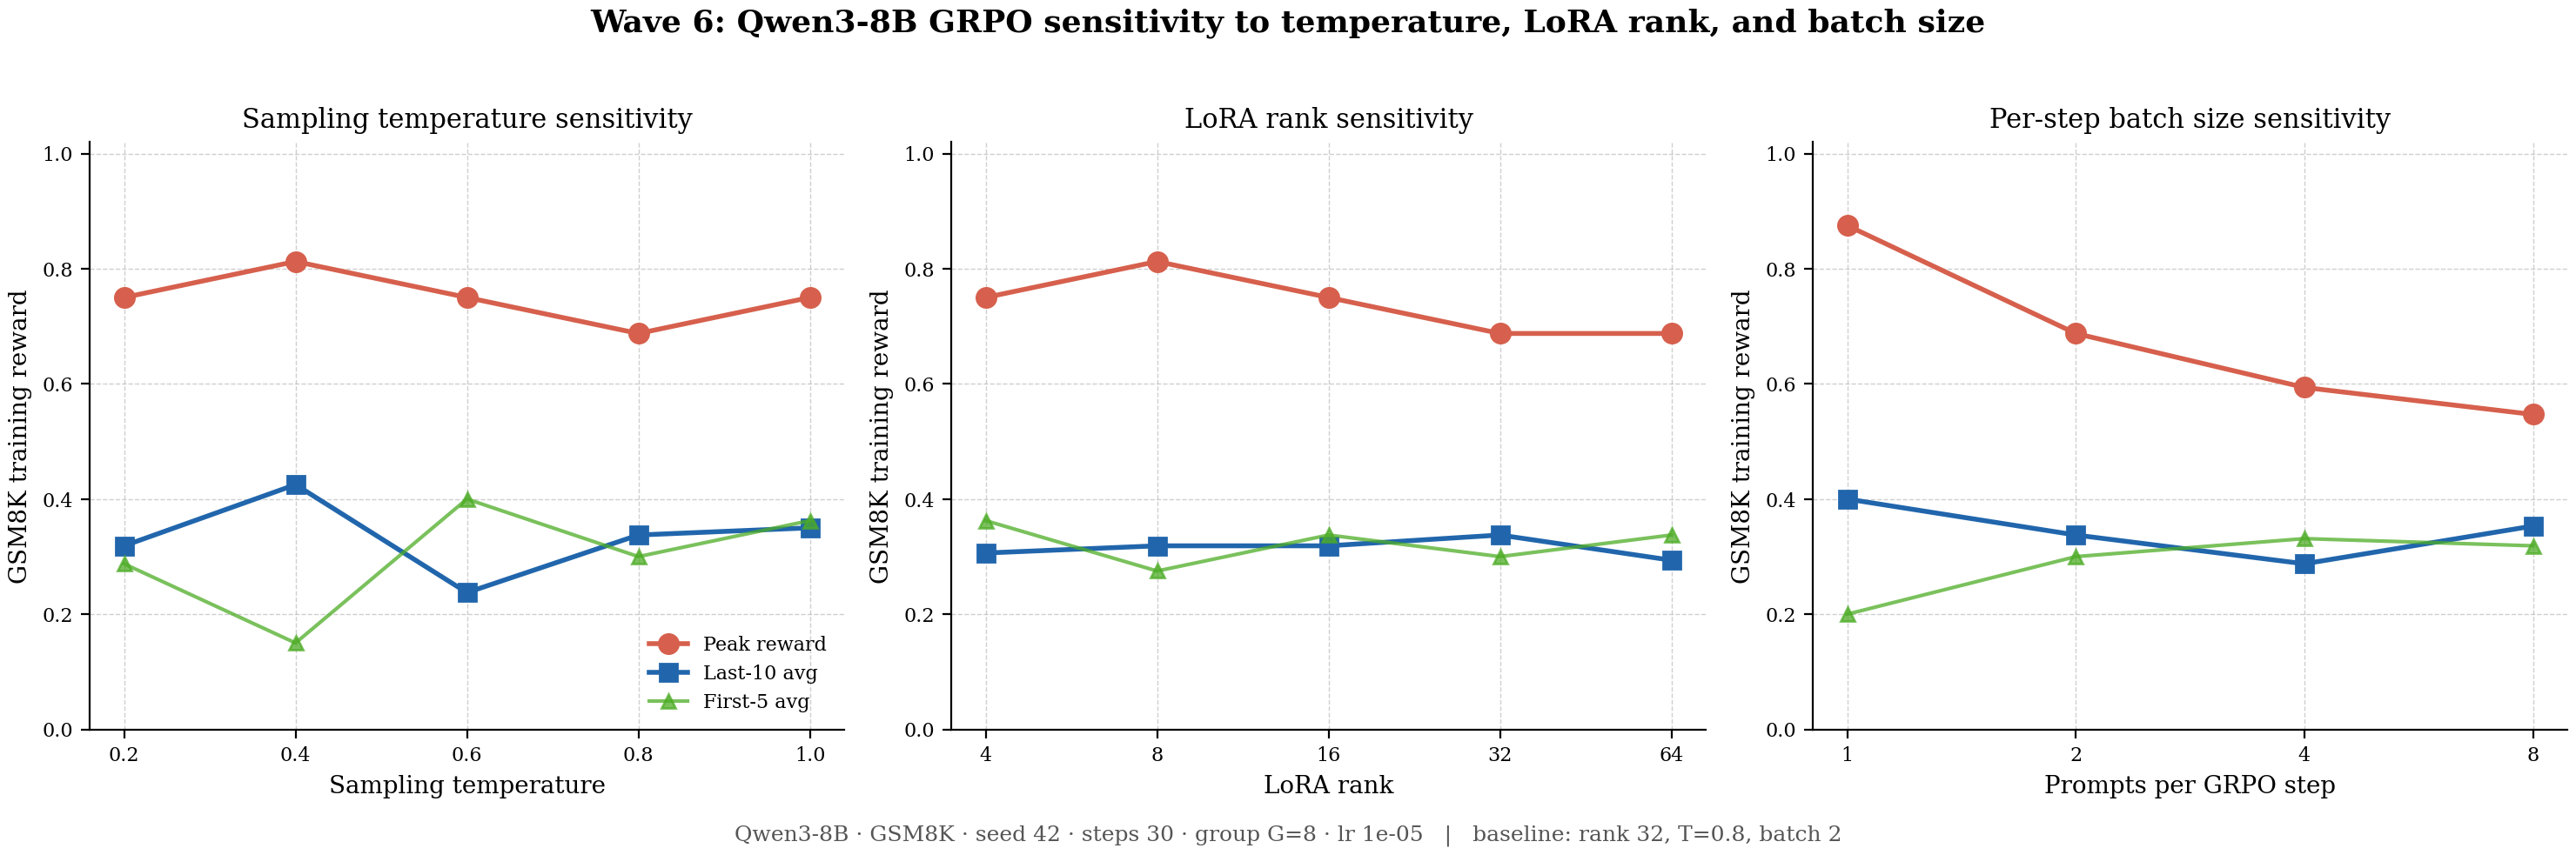
\includegraphics[width=\linewidth]{figures/wave6_sensitivity.png}
\caption{Wave~6 Qwen3-8B/GSM8K sweep (online training reward, one seed per
setting, 30 logged steps each). \textbf{Left:} temperature
$T\in\{0.2,0.4,0.6,0.8,1.0\}$. \textbf{Middle:} LoRA rank
$r\in\{4,8,16,32,64\}$. \textbf{Right:} per-step batch $B\in\{1,2,4,8\}$.
Circles: peak; squares: last-10 mean; triangles: first-5 mean.}
\label{fig:wave6_sensitivity}
\end{figure}

Peak reward lies in $[0.688,0.812]$ across temperature and the last-10 mean is
highest at $T=0.4$ (0.425); peak is $0.75$--$0.81$ for $r\le16$ and $0.688$ at
$r\in\{32,64\}$; across batch size the single-seed peaks are 0.875, 0.688,
0.594, and 0.547 for $B=1,2,4,8$ while the last-10 mean does not follow that
order. Peak-over-30-steps from one seed is a noise-dominated maximum, and
fixed-step runs at different $B$ spend different rollout budgets, so no
ordering or setting recommendation is claimed. At fixed policy and prompt
distribution $\mathbb{E}[B^{-1}\sum_{b=1}^{B}U_b]=\Pr(U=1)$ does not depend on
batch size; smaller batches change metric noise, not the expected mixed-group
fraction.

\subsection{Descriptive Observations From the Ledger}
\label{sec:ledger_obs}
The following are observations about single-run rows of
Table~\ref{tab:main_results}, not comparisons with identified causes.
\emph{Initialization:} the Qwen3-30B-A3B base row (5 logged points) peaks at
50\% while its instruct variant (3 logged points) peaks at 100\%; the row pair
cannot separate initialization from architecture, and short partial traces make
the gap descriptive only. \emph{Base checkpoints:} in campaign~v2 the base
checkpoints Llama-3.1-8B, Llama-3.1-70B, and DeepSeek-V3.1-Base have last-10
means of 8.8\%, 45.0\%, and 65.6\%, below the Kimi, GPT-OSS, and Qwen3.5 rows
of the same block, while the Qwen3-8B-Base executions are not; base-versus-instruct
status alone does not order these single runs, and no causal attribution to
instruction tuning is made. \emph{Non-monotone trace:} Nemotron-120B peaks at 87.5\% and
ends with a last-10 mean of 16.2\%, so a monotone saturation curve describes it
poorly; the trace does not identify a policy-level cause. \emph{Run-to-run
spread:} the two Qwen3-8B-Base executions differ by 13.1 points in last-10 mean
at identical visible settings, which bounds how much any single-run row can
carry.

% ---------------------------------------------------------------------------
\subsection{The Zero-Variance Fraction as a Reporting Field}
\label{sec:zvf-analysis}
% ---------------------------------------------------------------------------

The Zero-Variance Fraction at step $t$ is the fraction of sampled prompt groups
whose $G$ completions all receive identical rewards:
\[
  \mathrm{ZVF}_t = \frac{1}{|\mathcal{P}_t|}\sum_{p \in \mathcal{P}_t}
  \mathbf{1}\bigl[\operatorname{Var}_{c \sim \mathcal{C}(p)}\,r(c) = 0\bigr].
\]
When $\mathrm{ZVF}_t = 1$, every prompt has a zero centred reward-contrast
coefficient in the audited runner; this does not assert a zero total gradient.
The mixed-group fraction $1-\mathrm{ZVF}_t$ (historical alias GU) measures the
fraction of groups with nonconstant rewards, not gradient usefulness. We use
both strictly as descriptive reporting fields. Jointly with reward level, low
reward with high ZVF is a cold-start-like state and high reward with high ZVF a
possible saturation state, but unsigned ZVF does not choose an action, and no
early-warning, triage, or stopping value over reward level or slope is
measured here (Section~\ref{sec:withdrawn}).

\paragraph{ZVF theory.}
\label{sec:zvf-theory}
For binary rewards, let $p_{q,t}$ be the success probability for prompt $q$.
With conditionally independent completions and equal prompt weights,
\begin{align}
\widehat{\mathrm{ZVF}}_t &= \frac1{m_t}\sum_{q=1}^{m_t}
 \mathbf{1}\{\widehat{\operatorname{Var}}(r_{q,1:G})=0\},\\
\mathbb E[\widehat{\mathrm{ZVF}}_t\mid p_{1:m_t,t}]
 &=\frac1{m_t}\sum_{q=1}^{m_t}h_G(p_{q,t}),\quad
 h_G(p)=p^G+(1-p)^G.
\end{align}
For $G>1$, $h_G$ is symmetric and U-shaped, not monotone over $[0,1]$. At
$G=2$, $1-h_2(p)=2p(1-p)$ is twice the Bernoulli variance. The prompt average
of $h_G(p)$ is not $h_G(\bar p)$: at $G=8$, half the prompts at $p=0$ and half
at $p=1$ give mean reward $0.5$ and expected ZVF $1$, whereas all prompts at
$p=0.5$ give the same mean reward and expected ZVF $1/128$. Increasing $G$ from
8 to 16 at $p=0.2$ increases the expected mixed-group fraction by about 13.96
percentage points. The binary model is an assumption-dependent reference, not
empirical validation.

\paragraph{Why a linear reward control cannot show incremental information.}
Because the homogeneous-group probability is a nonlinear function of per-prompt
accuracy, a positive ZVF coefficient after a linear reward control need not
carry information beyond reward. At $G=2$, with $Z=2R^2-2R+1$ and $Y=R^2$,
$Y=-1/2+R+Z/2$ exactly: the coefficient on $Z$ repairs a misspecified linear
model although $Z$ is a function of $R$. Any predictive claim therefore needs
nonlinear reward/history baselines, whole-run holdout, and within-run dependence
handling; none is reported here.

% ---------------------------------------------------------------------------
\subsection{Withdrawn Displays}
\label{sec:withdrawn}
% ---------------------------------------------------------------------------
The binding standard of Section~\ref{sec:main_results} is applied to every
display of the earlier manuscript. The following are withdrawn; their values are
not reproduced here and support no claim of this audit.
\begin{itemize}[leftmargin=*,itemsep=1pt]
\item \emph{Reward-trajectory stability proxies (SI, PTD) over 28 experiments}
and the derived instability bins, algorithm means, and Nemotron case values: no
released per-run table identifies the 28 runs, windows, or zero-denominator
handling (targeted search of \texttt{platform\_hybrid/experiments/}), and PTD
$=1-\bar r_{\mathrm{tail}}/r_{\max}$ shares the tail mean with the outcome it was
correlated with, so the correlations are definitional rather than validating. The
accompanying KL-proxy figure is withdrawn with them. Definitions are in
Appendix~\ref{app:archive}.
\item \emph{Lagged ZVF partial correlations (``33 runs'')}: the stored output
\texttt{platform\_hybrid/experiments/zvf\_lagged\_regression\_results.json}
records counts and coefficients but no run IDs, and its generator
\texttt{zvf\_lagged\_regression.py} reconstructs 61 runs from the current tree
(58 at commit \texttt{ddcbb868}, where the output was last written), so the
33-run cohort cannot be bound. The table and the per-step ZVF heatmap are
withdrawn; only the counterexample above is retained.
\item \emph{Team proxy-task percentages} (restricted-sandbox ``HumanEval-style''
code, tool-calling, multi-stage reasoning) and the cross-architecture
tool-call schema percentages: no cell is bound to a run ID, evaluator revision,
window, or released artifact. The ``two-phase'' reward-pattern percentages and
the multi-seed consistency claim attached to them are withdrawn with them.
\item \emph{Campaign~v2 snapshot values} (Section~\ref{sec:main_results},
correction~ii) and the historical $G=8$ group-size row.
\item Earlier withdrawals retained as withdrawals: the 15-run cross-model ZVF
correlation, task-type ZVF means, scale correlation, and family ANOVA; the
selected-checkpoint GSM8K aggregate and scale summary; the saturation-fit
summaries; the scale scatter and model$\times$task heatmap; the arithmetic
cross-library comparison; and the historical significance families
(Appendix~\ref{app:archive}).
\end{itemize}

% =============================================================================
\section{Reproducibility}
\label{sec:reproducibility}
% =============================================================================

Reproduction is partial. Table~\ref{tab:availability-audit} separates local
implementation, backend configuration, and accessible evidence. The public
Hugging Face repositories named in the reviewed-cell manifest
(\texttt{platform\_hybrid/paper/manifests/p05\_reviewed\_cells\_manifest.json})
hold result JSON, step logs, and model cards at the recorded revisions; they do
not hold LoRA adapter weights. Tinker sampler checkpoints are identified only by
\texttt{tinker://} URIs on a managed service. W\&B is run-level metadata unless
a named export establishes step traces. No claim that all checkpoints or logs
are public is made.

\begin{table}[htbp]
\centering\small
\caption{Implementation and evidence availability by scope.}
\label{tab:availability-audit}
\begin{tabular}{p{.28\linewidth}p{.62\linewidth}}
\toprule
Scope & Availability and boundary \\
\midrule
Local runner & Reward processing and custom loss inspectable in source; version-specific \\
Managed configuration & Requested hyperparameters inspectable; execution identity requires logs \\
Server internals & Hardware placement, scheduling, and backend numerics undisclosed \\
Reviewed tool-use cells & Result/step-log files hashed and mirrored at fixed Hub revisions; raw group rewards and completions not stored \\
Ledger rows & Recomputed from the named repository artifacts by the ledger gate \\
Checkpoints & \texttt{tinker://} URIs only; no public adapter weights for the reviewed cells \\
Direct KL & Failed telemetry in affected runs; no recovered trace claimed \\
\bottomrule
\end{tabular}
\end{table}

% =============================================================================
\section*{Claims We Explicitly Do Not Make}
\label{sec:claims_we_do_not_make}

This is an audit of one heterogeneous run corpus, not a benchmark result, a new
algorithm, a new diagnostic, or a causal study. The runner omits the PPO
ratio/clip, the frozen reference policy, and the completion-only token mask; the
tool-use reward scores JSON schema rather than tool execution; and most runs are
single-seed and 10--30 steps long.
\begin{itemize}[leftmargin=*,itemsep=1pt]
\item We do not claim that this runner is canonical GRPO or that it improves reasoning, code, or tool use.
\item We do not claim that reward contrast, rather than algorithm labels, explains any cross-stack gap; no same-stack contrast manipulation was run.
\item We do not claim PPO-vs-GRPO, framework, dense-vs-MoE, or group-size rankings.
\item We do not claim that ZVF predicts final performance or that it is a validated triage diagnostic, early-warning signal, or stopping rule. Signed ZVF is a descriptive reporting field.
\item We do not claim a held-out GSM8K improvement. The separate five-adapter Qwen3-8B check (82.0\% base vs.\ 83.3\% mean) is a one-sample seed-level test against a fixed baseline, not a paired-seed test and not reviewed-record evidence ($p=0.26$).
\item We do not claim priority for the ZVF definition.
\end{itemize}

\section*{What We Do Claim}
\label{sec:what_we_claim}
(i)~For the specified runner, homogeneous rewards make the centred
reward-contrast term zero (Section~\ref{sec:diagnostic-method}).
(ii)~The two reviewed tool-use cells are all-wrong at every logged step, are
bound to hashed files and fixed Hub revisions, and do not identify their own
cause (Section~\ref{sec:evidence-identity}).
(iii)~Under one binding standard, the earlier ledger contained mislabelled
windows, snapshot values superseded by complete run-ID records, and summaries
with no released source; the corrected ledger and the withdrawal list are
Table~\ref{tab:main_results} and Section~\ref{sec:withdrawn}.

\section{Limitations}
\label{sec:limitations}
% =============================================================================

\paragraph{Noncanonical, partly opaque runner.}
The audited runner omits a probability ratio and clipping, a frozen reference
KL, and completion-only masking, and its loss includes prompt tokens under a
shifted target. Tinker is a managed, closed-source service: the local loss and
reward normalisation are inspectable, but server-side sampling, batching,
precision, and scheduling are not. Tinker rows measure a realised managed stack,
not canonical GRPO.

\paragraph{Short horizons, single runs, interruptions.}
Most rows are single runs of 10--30 steps; several stopped early because of
credential expiry or wall-clock limits and are reported only over their logged
steps. Two executions of one configuration differ by 13.1 points. The rows
support descriptive statements about early reward dynamics, not convergence,
rankings, or capability. The replication cautions of
\citet{henderson2018deep} apply.

\paragraph{Reviewed cells cannot be diagnosed.}
No raw completion or raw group-reward vector was stored for the reviewed cells,
so policy failure, parser strictness, and prompt-template mismatch remain
confounded (Section~\ref{sec:evidence-identity}).

\paragraph{Held-out evidence is narrow and contamination is possible.}
Only GSM8K has a held-out check, on 200 public test prompts with a single base
pass. GSM8K and HumanEval are public; the held-out split is held out from our
fine-tuning loop, not from the base models' pretraining.

\paragraph{Missing baselines and mechanism checks.}
No SFT-only warm start, best-of-$N$ or rejection sampling, DAPO/Dr.~GRPO-style
correction, or matched-budget dynamic-sampling arm was run, and the
fixed-completions reward-intervention check of Section~\ref{sec:discussion} was
not executed. These are the experiments a stronger claim would need.

\paragraph{Telemetry gaps.}
Direct KL tracking failed in the affected runs; response length and long-horizon
behaviour were not logged uniformly. Reward instability cannot be attributed to
drift, length bias, or reward hacking from these data.

\subsection{Broader Impact}
\label{sec:impact}
The artifacts are an audit and reporting contract, not a new capability; the
held-out evidence does not establish a capability change. Risks and data
provenance are in Section~\ref{sec:impact_standalone}.

% =============================================================================
\section{Discussion}
\label{sec:discussion}

\paragraph{What would make ZVF useful.}
An operator watching reward fixed at exactly zero for 30 steps already sees the
reviewed cells' failure; ZVF adds value only if it fires earlier, more
selectively, or more actionably than reward level or slope on runs that later
diverge. Testing that requires a frozen signed-ZVF rule evaluated on held-out
whole runs against flexible reward mean/slope/history baselines, with false
stops and recoveries counted.

\paragraph{Mechanism check (not executed).}
Hold policy, sampled completions, and token masks fixed and intervene on reward
vectors to verify centred coefficients and their reward-gradient contribution in
the deployed runner. This is distinct from randomising prospective sampling
policies over a common task population at matched budgets.

\paragraph{Prespecified evaluation of a diagnostic policy (future work).}
Compare continuing the fixed schedule, a declared dynamic-sampling/retry rule,
and the proposed diagnostic policy using common initialisations, tasks,
evaluators, and a fixed generation budget. Charge discarded and resampled
completions, token lengths, and any warm-start training to that budget.
Measure held-out quality at budget exhaustion, expenditure, false stops, and
recovery; include all-failure groups with correct and malformed verifiers,
all-success groups, mixed groups without improvement, and initially
unproductive runs that later recover. Compare flexible reward mean/slope/history
baselines with all-wrong/all-correct fractions, success-count distributions,
and advantage variance before attributing incremental value to ZVF.
Independent training seeds are the replication unit; sample size follows a
prespecified effect or precision target and adequate failure-event coverage.
At $G=8$, $h_8(0.2)=h_8(0.8)\simeq0.168$ and $h_8(0.25)\simeq0.100$, so
25\%/75\% pass-rate cutoffs do not define near-degenerate groups; such a regime
should be defined through a prespecified target $h_G(p)$. No such prospective
result is reported here.

\paragraph{Prior and concurrent interventions.}
Zero-advantage dead zones motivate prompt pre-screening such as
AERO~\citep{zhang2026aero}; TPO~\citep{kaddour2026tpo} yields a zero
first-epoch reward-directed gradient for homogeneous groups at the rollout
snapshot; and \citet{wu2025grpodpo} relate GRPO and DPO contrastive
representations under stated assumptions. The two reviewed all-wrong cells do
not calibrate, validate, or rank any of these.

% Conclusion (shared with archived roots; unchanged)
\section{Conclusion}
\label{sec:conclusion}
This audit establishes a scoped centered-reward identity, records two descriptive
all-wrong synthetic tool-use cells, and specifies the evidence needed to interpret
heterogeneous post-training observations. It does not establish intervention
benefit, a stopping rule, or an algorithm ranking. Conflicting historical cohorts
remain unresolved rather than being reconciled by selecting a plausible value.
The next empirical question is whether a prespecified operator policy improves
held-out outcomes at a matched budget, compared with reward/history baselines
on independent held-out runs. That experiment has not been demonstrated here.


% Ethics, limitations, and broader impact: paper-05 fork of ethics_statement.tex
% =============================================================================
% Ethics Statement and Broader Impact -- paper-05 fork (2026-10-19 ARS revision)
% Forked from ethics_statement.tex, which ethics_wrapper.tex and the archived U01
% roots still use; edit this file for platform_hybrid/paper/paper.tex only.
% Intended placement: after the Conclusion section, before References.
% Label: \label{sec:impact_standalone}
% Target length: >= 2 pages (NeurIPS Broader Impact guidance).
% =============================================================================

\section{Ethics, Limitations, and Broader Impact}
\label{sec:impact_standalone}

This statement complements Section~\ref{sec:limitations} with a dual-use
analysis, the status of compute and carbon accounting, data provenance, the
closed-source training backend, and methodological limits we did not close.

% ---------------------------------------------------------------------------
\subsection{Dual-Use Analysis: Misuse Risks of Reasoning RL}
\label{sec:dualuse}
% ---------------------------------------------------------------------------

\paragraph{Threat model.}
\ours{} releases (i) training scripts that apply GRPO to the GSM8K
\cite{cobbe2021training} mathematical reasoning benchmark and to the
Salesforce xLAM-Function-Calling-60k \cite{liu2024xlam} tool-use corpus,
(ii) twelve public Hugging Face repositories
\texttt{arvindcr4/tinker-rl-bench-<tag>}, enumerated with their revisions in
\path{platform_hybrid/paper/manifests/p05_hub_repositories.json}; ten hold only
result JSON, step logs, and model cards, and two
(\texttt{ppo\_gsm8k\_Qwen3-8B\_s42}, \texttt{ppo\_gsm8k\_Llama-3.1-8B-Instruct\_s42})
hold LoRA adapter weights from the Modal PPO runs, and (iii) diagnostic code for
Zero-Variance Fraction, reward-stability, and length-bias analysis. We
analyse four concrete misuse pathways these artefacts could, in principle,
enable, and we describe the existing guardrails and the residual risk we
judge acceptable for publication.

\paragraph{M1. Weaponisation of mathematical reasoning.}
The most capability-relevant artefact we release is GRPO training code evaluated
on grade-school arithmetic and multi-step reasoning; the reviewed evidence is
inconclusive about a capability improvement. A malicious
operator could attempt to extend this pipeline to tasks of greater
dual-use concern, e.g., chemistry olympiad problems, cryptographic key
recovery, or financial fraud. We judge the \emph{marginal} uplift provided
by our release to be small for three reasons. First, no capability change is
established: the base Qwen3-8B checkpoint already scores 164/200 on the
held-out GSM8K slice, and the separate five-adapter check
(Section~\ref{sec:heldout}) is inconclusive. Its seed-level difference is not
a bound on capability change, which remains unmeasured within wide uncertainty
(single base pass, no baseline variance); ``inconclusive'' does not establish
``small uplift''.
Second, the public literature already contains GRPO implementations
\cite{shao2024deepseekmath, openrlhf2024, verl2024, vonwerra2022trl} that are at
least as capable. Third, any reasoning uplift is bounded by the rewarder:
GSM8K rewards use exact-match against a human-written gold answer, which
does not generalise to the domains listed above without a new reward
signal, which itself requires expertise and labelled data.

\paragraph{M2. Reward hacking and the long-term alignment risk.}
GRPO, like all policy-gradient RL from a proxy reward, is vulnerable to
reward hacking: the model learns to exploit idiosyncrasies of the reward
function rather than solve the intended task \cite{skalse2022specificationgaming,
krakovna2020specification}. Length and long-horizon
behaviour were not logged uniformly (Section~\ref{sec:limitations}), so reward
hacking is neither demonstrated nor excluded.
Users who apply our scripts to under-specified reward functions in
production settings (e.g., a custom ``helpfulness'' classifier) may observe
models that appear to improve on held-out metrics while silently
optimising against unintended proxies. We include the Zero-Variance
Fraction and reward-stability diagnostics precisely as retrospective summaries; they do not identify policy drift or reward hacking.

\paragraph{M3. Circumventing safety training via distillation or tool-use.}
The tool-use track trains LoRA adapters that teach a base model to emit
schema-valid JSON function calls \cite{liu2024xlam}. A motivated adversary
could in principle use the same pipeline to teach a base model to emit
jailbreak prompts as ``tool calls'' or to invoke an adversarial external
tool. We mitigate this by (a) not releasing adapter weights for the tool-use runs
(the corresponding Hub repositories hold result metadata only) and releasing only
adapters, not merged weights, elsewhere,
while noting that an adapter can still alter safety behavior and does not
guarantee that instruct-model safeguards remain effective; (b) stating here that the tool-use runs used a narrow schema (five
synthetic tools) and were not safety-evaluated for open-ended function
calling; and (c) not releasing any function-calling harness that would
actually execute emitted calls.

\paragraph{M4. Compute-efficiency externalities.}
This audit makes no demonstrated efficiency claim or group-size recommendation. Improved training efficiency is
itself dual-use: it lowers the cost of running adversarial fine-tuning at
scale. We judge this externality to be modest relative to the already-low
cost of fine-tuning a 0.6B--8B model with commodity LoRA recipes
\cite{hu2022lora}, but we flag it explicitly.

\paragraph{Residual risk.}
After weighing M1--M4 we judge that the reproducibility, calibration, and
pedagogical benefits of releasing \ours{} outweigh the residual misuse
risk. We adopt the standard mitigation of releasing adapters (not merged
weights), documenting intended use and out-of-scope use in model cards,
and publishing alongside the diagnostics a researcher would need to detect
reward hacking.

% ---------------------------------------------------------------------------
\subsection{Compute Cost Accounting}
\label{sec:compute_accounting}
% ---------------------------------------------------------------------------

No reconciled spend ledger exists. The historical platform entries (retained,
for audit only, in the shared \path{platform_hybrid/paper/ethics_statement.tex})
are mutually inconsistent: excluding Colab, their numeric ranges sum to USD
147--177 against an earlier stated USD 130--140 total, and cash versus credits,
dates, cohort overlap, and failed-run inclusion are unreconciled. We therefore
report no spend figures and no project total.

\paragraph{Hidden costs.} Beyond direct platform spend, the project
consumed human labour (approximately six student-FTE-months, unpaid) and
infrastructure generously subsidised by PES University's LLM Research
Group (shared access to one A100 node used for TRL baselines and
pre-submission sanity checks). No author received commercial compensation
from Thinking Machines, Modal, or any other vendor mentioned.

\paragraph{Failed-run accounting.} Some spend was consumed by runs that
failed (JWT expiry, API stalls for GPT-OSS-20b and Kimi-K2 before re-run, the
KL-tracking gradient bug); the failed-run subset is not reconciled, so no
amount is stated.

% ---------------------------------------------------------------------------
\subsection{Carbon Footprint Estimation}
\label{sec:carbon}
% ---------------------------------------------------------------------------

No measured energy or emissions data exist for this project. Tinker does not
disclose hardware allocation or GPU-hours, and the historical Modal GPU-hour
figures conflict (18 versus 250 GPU-hours in different summaries). Earlier
versions tabulated conditional scenarios (TDP $\times$ assumed hours $\times$
PUE $\times$ grid intensity, following \citet{patterson2024empirical} and
\citet{strubell2019energy}); because their hours are unreconciled and their
accelerator counts assumed, any summed total would be read as a footprint it is
not, so no carbon figure is reported. A future release needs a single ledger
with dates, cohort IDs, GPU counts, measured versus assumed hours, and failure
status before reporting totals.

\paragraph{Offset and mitigation.}
We did not purchase carbon offsets. Instead, we have (a) published run
result files and step logs (Section~\ref{sec:reproducibility}) so that
downstream users need not re-run the experiments to inspect them; (b) retained local step-level CSV logs so that
learning curves can be inspected without re-training; and (c) listed the failed and quarantined runs, so that
replicators can skip them. We regard reproducibility-by-artefact as a
more durable mitigation than offsets.

% ---------------------------------------------------------------------------
\subsection{Data Provenance}
\label{sec:provenance}
% ---------------------------------------------------------------------------

\ours{} uses only publicly released research datasets. No private data,
personally identifiable information, or licensed proprietary content is
used. No human annotators were employed during this work. We document
each dataset below.

\paragraph{GSM8K \cite{cobbe2021training}.}
Grade-school math word problems (7{,}473 train / 1{,}319 test)
authored by human writers contracted by OpenAI. Released under the
\textbf{MIT License} via \url{https://github.com/openai/grade-school-math}.
We use the standard train/test splits without modification. The canonical
citation is \citet{cobbe2021training}. Known limitations of GSM8K include
gender-neutral but culturally US-centric word problems (names, currencies,
sports) and a moderate rate of human-labelling errors estimated at
\textasciitilde 2\% by \cite{zhang2024gsm1k}. Our held-out evaluation
respects the test/train split.

\paragraph{Salesforce xLAM-Function-Calling-60k \cite{liu2024xlam}.}
60{,}000 function-calling examples generated by Salesforce Research as
training data for the xLAM agentic model family. Released under the
\textbf{CC BY 4.0} license via \url{https://huggingface.co/datasets/Salesforce/xlam-function-calling-60k}.
We use the public release as-is in tool-use tracks of the broader corpus; no
xLAM-based result is displayed in this audit.
Known limitations: xLAM schemas are synthetic and skew toward cleanly-typed
arguments; the dataset under-represents ambiguous, error-handling, and
multi-turn tool-calling. Attribution to Salesforce is required by the
license and is provided in Section~\ref{sec:acknowledgments} and in the
xLAM-derived model cards.

\paragraph{HumanEval \cite{chen2021codex}.}
164 Python programming problems with unit tests, released by OpenAI under
the \textbf{MIT License}. The local restricted sandbox does not implement an unmodified standard
pass@$k$ evaluation; code results are harness-bound reward probes. Known
limitations: small scale, English-language docstrings, single-language
coverage; documented contamination concerns against frontier pretraining
corpora \cite{riddell2024contamination}.

\paragraph{NuminaMath \cite{li2024numinamath}.}
Used by collaborator Mohammad Rafi for the multi-stage
GSM8K+NuminaMath pipeline. Released under \textbf{Apache 2.0}. We use a
downstream checkpoint reported by Rafi; our repository contains only his
scripts and the Apache-licensed derivative weights.

\paragraph{Open-Platypus \cite{lee2023platypus}.}
3{,}000 SFT examples used by collaborator Madhu for Qwen3-8B code
generation warm-up. Open-Platypus is a curated subset released under
\textbf{CC BY-NC 4.0}; the non-commercial restriction is respected in our
release, which is academic-use only.

\paragraph{Synthetic tool-use prompts (authored).}
The reviewed all-wrong cells use ten authored requests over five synthetic tools
(calculator, weather, search, reminder, translate) defined in the candidate
runner source (Section~\ref{sec:evidence-identity}; hash in the reviewed-cell
manifest). An earlier version of this statement described a different five-tool
corpus under \texttt{data/synthetic\_tools/}; no such directory exists in the
repository, and that description is withdrawn. No user data, scraped web
content, or proprietary API traces are present.

\paragraph{No web scraping, no human subjects.}
We did not scrape any website. We did not run any study with human
participants. No IRB review was therefore required. No data that could
reasonably be considered to contain PII, copyrighted content, or sensitive
personal attributes was used at any stage of training, evaluation, or
reward modelling.

% ---------------------------------------------------------------------------
\subsection{Closed-Source Tinker Acknowledgment}
\label{sec:tinker_closed}
% ---------------------------------------------------------------------------

A central tension in \ours{} is that a substantial fraction of our
headline numbers come from a closed-source commercial platform while our
paper simultaneously advocates for reproducibility and platform
independence. We do not resolve this tension by hiding it; we describe
it precisely.

\paragraph{What Tinker is and is not.}
Tinker \cite{thinkingmachines2024tinker} is a managed LLM fine-tuning and
inference service provided by Thinking Machines, Inc. It exposes a Python
SDK (stated elsewhere as \texttt{tinker==0.16.1}; the Hub model cards of the
reviewed cells state v0.18.1, and the executed version is not bound) that accepts custom loss functions
(\texttt{forward\_backward\_custom}), a limited set of optimisers, and
standard LoRA hyperparameters. Local scripts specify reward normalization, baseline subtraction, custom loss,
and requested LoRA/optimizer configuration. Undisclosed server-side details
include hardware placement, scheduling, execution numerics, and some batching
and sampler behavior. These are separate from the inspectable local objective.

\paragraph{What this means for our claims.}
We have not ruled out seed variance, checkpoint/model-size confounding, evaluator
differences, or backend effects. The arithmetic/GSM8K cross-library identity is
unresolved. Tinker results do not establish an upper bound or algorithmic
superiority. verl/OpenRLHF Task~4 dry runs are engineering artifacts, not
measured alternatives. The contribution remains the centered-reward identity,
descriptive audited cells, and reporting contract.

\paragraph{Reproducibility commitments we can make.}
Section~\ref{sec:reproducibility} distinguishes local source, observed
configuration, undisclosed internals, and evidence access. A dagger denotes only
interrupted execution; backend provenance is stated explicitly. Exact checkpoint
revisions and public access must be verified per artifact; no blanket release
or future rerun commitment is made here.

\paragraph{Key rotation and credential hygiene.}
Our Tinker API key (prefix \texttt{tml-...}) is held in a repository
\texttt{.env.example} placeholder only. The real key is stored in the
authors' password manager and rotated whenever a failure mode suggests
possible exfiltration. No Tinker key is committed to git history in
either the primary repository (\texttt{pes-llm-research/tinker-rl-lab}) or
the mirror (\texttt{arvindcr4/tinker-rl-lab}).

% ---------------------------------------------------------------------------
\subsection{Known Methodological Limits}
\label{sec:methodlimits}
% ---------------------------------------------------------------------------

In addition to the infrastructure failures and platform-specific caveats
enumerated in Section~\ref{sec:limitations}, we flag the following
methodological limits.

\paragraph{Short training horizons.}
Most reviewed Tinker runs have short, often 30-step horizons; this is not
a universal limit for all later scripts or campaigns. This is a
deliberate cost-control choice and means our Tinker numbers are
\emph{early-training snapshots}. We cannot rule out that longer training
would change the qualitative picture. The separate held-out GSM8K check (Section~\ref{sec:heldout}) is a
one-sample seed-level test against a fixed baseline, not paired-seed and not
reviewed-record evidence; it establishes no held-out gain.

\paragraph{Single-seed Tinker experiments.}
Each Tinker configuration in the ledger was run once, except Qwen3-8B-Base,
whose two executions at the same visible settings differ by 13.1 points in
last-10 reward; best practice prescribes 3--5 runs \cite{henderson2018deep}. Tinker results therefore lack
variance estimates and do not support significance testing; we report
them descriptively. Seed-level inference requires the actual independent seed observations and
an identified estimand; reconstructed seed vectors are not eligible.

\paragraph{Train-set reward as primary Tinker metric.}
Tinker runs primarily report reward on training prompts. Only the GSM8K
track was followed up with a separate 200-example held-out evaluation
per seed. Other Tinker tracks (tool-use, xLAM) remain train-set-only and
we cannot distinguish memorisation from generalisation for those
settings.

\paragraph{LoRA only; no full fine-tuning.}
The reviewed LLM fine-tuning runs use LoRA \cite{hu2022lora}, with settings
varying by cohort; the Wave~6 rank sweep also includes rank 4. We have
\emph{not} tested whether full fine-tuning would re-order the
library/algorithm comparisons. The LoRA constraint is practical (cost) but
it means our claims about PPO vs.\ GRPO and TRL vs.\ Tinker are
LoRA-conditional.

\paragraph{Benchmark coverage is narrow.}
The broader corpus touches GSM8K, MATH-500 (exploratory), HumanEval
(subset), and synthetic/xLAM tool use; this audit displays only GSM8K and the
synthetic tool-use cells. We do not evaluate on MT-Bench,
ArenaHard, safety benchmarks (HarmBench, ToxicChat), or truthfulness
benchmarks (TruthfulQA). Any claim about ``reasoning'' in the paper is
strictly a claim about the covered benchmarks.

\paragraph{No human preference data.}
We use verifiable rewards only (exact-match for math, unit-test for code,
schema-validity for tool-use). We do not study RLHF with human preference
data; findings should not be extrapolated to reward-model--based alignment
without further work.

\paragraph{Closed-source implementation opacity (reiterated).}
Comparisons between Tinker GRPO and TRL GRPO are confounded by the
closed-source nature of Tinker's implementation. See
Section~\ref{sec:tinker_closed} for detail.

\paragraph{Cross-platform hardware confounding.}
Tinker, Modal, Colab, and the PES A100 node use different accelerators,
different memory hierarchies, and different inference/training stacks
(Tinker proprietary, Modal vLLM, Colab PyTorch-native, TRL+Accelerate).
Observed differences in reward dynamics are not purely algorithmic.

\paragraph{Carbon estimates are approximate.}
As discussed in Section~\ref{sec:carbon}, Tinker GPU-hour and TDP are
inferred, not measured. Grid intensity is region-average, not marginal.
No carbon figure is reported for that reason.

\paragraph{Exploratory, not confirmatory.}
This is an exploratory case study, not a pre-registered confirmatory
experiment. We did not pre-register primary hypotheses. The conflicting historical correction families and step-based significance
decisions are withdrawn (Section~\ref{sec:statistical-policy}); exploratory
coefficients do not establish calibrated inference.

\paragraph{Geographic and demographic limits.}
All authors are based at a single institution in Bengaluru, India. Our
choice of benchmarks, prompt phrasings, and evaluation design reflects
that context. Independent replication by groups in other regions, on
non-English tasks, and with non-Qwen / non-Llama families is an open
question.

% =============================================================================
% End of ethics_statement.tex


\begin{ack}
\label{sec:acknowledgments}
We thank our project guides \textbf{Prof.~Narayana Darapaneni}
(Northwestern University / Great Learning) and
\textbf{Mr.~Anwesh Reddy Paduri} (Great Learning / PES University)
for their mentorship and technical guidance throughout this capstone project.
We thank the Tinker team for API access and the Modal team for GPU compute credits
(H100 cluster). We thank Weights \& Biases for experiment tracking infrastructure
and Hugging Face for model hosting. This work was supported in part by PES
University's LLM Research Group. We are grateful to the open-source communities
behind TRL, Stable Baselines3, CleanRL, Tianshou, OpenRLHF, veRL, and the
broader Hugging Face ecosystem.
Artificial intelligence was also used as a tool in manuscript preparation.
\end{ack}

% =============================================================================
% References (no \nocite: only cited entries of the shared references.bib print)
% =============================================================================
\bibliographystyle{plainnat}
\bibliography{references}

% =============================================================================
\appendix
% =============================================================================

\section{Archival Correction Log}
\label{app:archive}

This appendix records, once, what the earlier manuscript contained and why it is
no longer displayed. It is an audit log for readers of the earlier text, not
additional evidence.

\paragraph{Configuration inventories.}
The earlier text listed library mappings (TRL, Stable Baselines3, CleanRL,
Tianshou, PufferLib, rl\_games, d3rlpy), a classic-RL PPO hyperparameter
mapping, a PPO sweep grid, a task-taxonomy diagram, a pipeline diagram, and a
feature comparison with Gymnasium, SB3 Zoo, CleanRL, and Dopamine. Only TRL,
SB3, CleanRL, and Tianshou produced reported runs; the classic-RL PPO runs
reached near-zero reward on a tokenized-text arithmetic task, which shows stack
mis-specification, not a property of PPO. None of these inventories supports a
claim and they are omitted.

\paragraph{Withdrawn analyses and their reasons.}
(a)~\emph{Arithmetic cross-library comparison}: its TRL five-seed score is also
labelled five-seed GSM8K on Qwen2.5-0.5B, and its Tinker row is
summary-statistics-only, reconstructed for bootstrap analysis; no common-task
seed cohort exists. The five-seed TRL cross-seed figure inherits the same
task-label conflict and is omitted.
(b)~\emph{GSM8K scale summary}: its values exist only as a hand-entered
dictionary (\texttt{GSM8K\_SCALING} in
\texttt{platform\_hybrid/experiments/compute\_statistics.py}, recording $n=10$
rather than five seeds), and the corresponding W\&B runs for Qwen3-0.6B and
Qwen3-14B are recorded as failed.
(c)~\emph{Selected-checkpoint aggregate}: ten checkpoints chosen by high
training reward; their held-out rows are a selection analysis, not comparable
with the reviewed record.
(d)~\emph{Scale scatter and model$\times$task heatmap}: mixed training reward
with held-out accuracy, duplicated labels, and cells that did not match the
ledger.
(e)~\emph{Saturation fits}~\citep{nimmaturi2025predictive}: text and figure
versions disagreed on trace count (44 vs.\ 28), mean $R^2$, and correlations;
the released \texttt{platform\_hybrid/experiments/fit\_saturation\_model.py}
fits a different parameterisation and reports no $R^2$.
(f)~\emph{Group-size panel}: pooled \texttt{campaign\_v2\_w2\_*},
\texttt{campaign\_v2\_w1\_qwen3-8b-base}, and \texttt{scale\_gsm8k\_qwen3-8b}
at $G=8$; not one cohort.
(g)~\emph{Significance families}: historical five-test, 20-test BH, and
38-test Bonferroni families were inconsistent and used step-iid inference
(Section~\ref{sec:statistical-policy}).
(h)~\emph{BrowserGym/MiniWoB smoke run}: a one-step integration check with 0.0
reward and zero trainable groups; integration evidence only.

\paragraph{Stability-proxy definitions (values withdrawn).}
For completeness: the Stability Index was the coefficient of variation of the
last-10 rewards, $\sigma(r_{\text{tail}})/|\mu(r_{\text{tail}})|$; Peak-to-Tail
Drift was $(r_{\max}-\bar r_{\text{tail}})/r_{\max}$; both are undefined at zero
denominators, and an all-zero trace is an all-zero reward state, not a stability
classification.

% Deterministic analytical checks (section file used only by this root)
\section{Analytical Regression Cases and Release Gates}
\label{app:audit-regressions}
These cases are deterministic mathematical checks, not additional experimental
observations. They guard the interpretations above without training or changing
stored result artifacts.
\begin{enumerate}
\item For any constant reward vector and $\epsilon>0$, each
$(r_i-\bar r)/(s+\epsilon)=0$. For $(0,1)$ with population SD $1/2$, the
coefficients are $\mp (1/2)/(1/2+\epsilon)$. This tests coefficients, not a
nonzero total gradient or a learning benefit.
\item For $G=8$, $h_G(0)=h_G(1)=1$ and $h_G(1/2)=1/128$.
Two prompt populations with mean success $1/2$ can therefore have expected
ZVF $1$ and $1/128$, respectively. At $p=0.2$, the GU gain from $G=8$ to
$16$ is approximately $0.1396272$.
\item At $G=2$, $1-h_G(p)=2p(1-p)$. For $Z=2R^2-2R+1$ and $Y=R^2$,
$Y=-1/2+R+Z/2$ exactly. A nonzero ZVF coefficient after a linear reward
control need not represent new predictive information.
\item For homogeneous TPO scores, $q=p_{\mathrm{old}}$; at the rollout snapshot,
$p_\theta-q=0$. This does not exclude anchoring after other groups update the
policy on later epochs.
\item For an all-zero reward trace, both SI and PTD have zero denominators and
Cohen's $d$ has zero pooled variance. All are undefined, not zero-valued evidence
of stability or no effect.
\item The listed non-Colab spend ranges sum to USD 147--177, not USD 130--140.
This is an arithmetic audit of historical entries, not a verified expenditure.
\item Even hypothetical perfect detection of two independent positive cases
would give a two-sided exact 95\% sensitivity interval
$[\sqrt{0.025},1]\simeq[0.158,1]$. This is a conditional binomial
illustration, not a recovered confusion matrix or a validated trigger.
\item Convexity gives $\mathbb E_x[h_G(p_x)]\ge h_G(\mathbb E_x[p_x])$
for $G\ge2$. Replacing latent $p_x$ by finite-sample estimates introduces
estimation error and nonlinear plug-in bias; the population bound does not
certify an empirical residual explanation.
\end{enumerate}

\paragraph{Required release checks, not a certification.}
A release should resolve every included reference/citation and required asset;
render and inspect the PDF; reject significance output for ineligible records
and seed bootstraps based on reconstructed observations; enforce shared family
IDs across displays; and exclude quarantined or dry-run rows from empirical
plots. A manifest must tie the PDF hash, source commit, immutable cohorts,
analysis version, and figure hashes together. This source-only correction does
not regenerate figures or assert that the existing generators implement these
gates. The historical statistical appendix is excluded from this root; its
source remains an archived generated artifact requiring generator-side repair.


% =============================================================================
% NeurIPS-style checklist (paper-05 fork of sections/checklist.tex)
% =============================================================================
% Paper-05 fork (2026-10-19) of sections/checklist.tex, which the archived U01
% roots also use. Checklist for the audit manuscript, not the historical claim list.
\section*{NeurIPS Paper Checklist}
\begin{enumerate}
\item \textbf{Claims.} Do the main claims reflect the contributions and scope?
\answerYes{The abstract, introduction, and claims sections use the same three
contributions: a centered-reward identity for the specified runner, an
artifact-bound audit of the two reviewed cells, and a ledger re-audit under one
binding standard. No algorithm ranking, validated triage or stopping rule,
independent predictive signal, or intervention benefit is claimed.}

\item \textbf{Limitations.} Are limitations discussed?
\answerYes{Section~\ref{sec:limitations} addresses the noncanonical objective,
short horizons, missing replications, proxy rewards, backend opacity, and missing
telemetry. Section~\ref{sec:evidence-identity} lists unresolved cohorts.}

\item \textbf{Theory assumptions and proofs.} Are assumptions and derivations stated?
\answerYes{Section~\ref{sec:diagnostic-method} specifies the local loss and the
centered-coefficient identity. Section~\ref{sec:zvf-theory} distinguishes empirical
ZVF from its conditional Bernoulli expectation. Appendix~\ref{app:audit-regressions}
gives deterministic checks. No zero-total-gradient or learning-benefit theorem
is claimed.}

\item \textbf{Experimental result reproducibility.} Is all needed information disclosed?
\answerNo{Local implementation is inspectable and ledger rows are recomputed
from named artifacts by a gate script, but execution-to-source mappings,
checkpoint revisions, server internals, and raw group rewards are not available.
Table~\ref{tab:availability-audit} records the boundaries.}

\item \textbf{Open access to data and code.} Are reproduction artifacts openly accessible?
\answerPartial{Source, the cited result files, and twelve public Hub
repositories (exact names and revisions in
\texttt{manifests/p05\_hub\_repositories.json}) are available; ten hold
result metadata only. No blanket checkpoint or telemetry availability is
certified.}

\item \textbf{Experimental setting/details.} Are relevant settings specified?
\answerPartial{Nominal configurations and cohort-specific exceptions are described;
missing run revisions, logging-window definitions, and backend details remain
explicitly unresolved. Five-seed replication does not apply to every experiment.}

\item \textbf{Experiment statistical significance.} Are uncertainty and inference appropriate?
\answerNo{The historical step-iid tests, synthetic-seed bootstrap intervals, and
inconsistent correction-family decisions are withdrawn. This audit supplies
descriptive observations and a future eligibility policy, not new inferential
results (Section~\ref{sec:statistical-policy}).}

\item \textbf{Experiments compute resources.} Are resource requirements fully reported?
\answerNo{No reconciled spend or GPU-hour ledger exists.
Section~\ref{sec:compute_accounting} records the arithmetic discrepancy and
Section~\ref{sec:carbon} why no carbon figure is reported.}

\item \textbf{Code of ethics.} Is ethical compliance discussed?
\answerPartial{Section~\ref{sec:impact_standalone} discusses foreseeable misuse,
reward hacking, data provenance, and uncertainty. This checklist does not certify
unverified artifact-release or license completeness.}

\item \textbf{Broader impacts.} Are positive and negative impacts discussed?
\answerYes{The ethics statement discusses research accessibility and potential
misuse. Neither capability uplift nor compute-saving benefit is established.}

\item \textbf{Safeguards.} Are appropriate safeguards described?
\answerPartial{Tool-schema scores do not establish safe tool execution. Adapter
release does not preserve safety guarantees; open-ended tool use and safety
benchmarks have not been evaluated.}

\item \textbf{Licenses for existing assets.} Are assets credited and licenses stated?
\answerPartial{Section~\ref{sec:provenance} lists dataset sources and reported
licenses. Exact revisions and downstream restrictions need artifact-specific
verification before redistribution.}

\item \textbf{New assets.} Are new assets documented?
\answerPartial{The synthetic prompts, reward, and local objective are described
and hashed in \texttt{manifests/p05\_reviewed\_cells\_manifest.json};
execution-commit binding, raw group rewards, and checkpoint revisions remain
unbound.}

\item \textbf{Crowdsourcing and human subjects.} Are participant details supplied?
\answerNA{No new human-participant study or crowdsourcing is reported.}

\item \textbf{IRB approvals.} Is an applicable approval documented?
\answerNA{No new human-participant study is reported; this is not a claim of
formal institutional review of every downstream use.}

\item \textbf{LLM usage.} Is use of LLMs disclosed?
\answerYes{LLMs are the subject of the experiments, and AI assistance in
manuscript preparation is disclosed in the acknowledgments.}
\end{enumerate}


\end{document}
